% \newcommand{\vect}{\boldsymbol}
% \newcommand{\vect}{\mathbf}

\chapter{二维材料 Chern 数算法}

考虑无限大二维材料的布里渊区(Brillioun Zone,简称BZ),其由两个实参数刻画,$\{k_x, k_y\}$,也即准动量$\vect{k}=(k_x, k_y)$。参数空间为 Torus 结构 (以下简称$T^2$),即 $k_x\in[0, 2\pi]$, $k_y\in[0, 2\pi]$,且 0 与 $2\pi$ 等价。考虑该材料的某一能带,引入其波函数记作 $|u(\vect{k})\rangle$,则陈数(以下称 Chern 数)刻画了一个从该 Brillioun 区($T^2$)上的到一个球面(以下简称$S^2$)的映射:

\begin{align}
T^2 \rightarrow S^2 : C = \frac{1}{2\pi}\int_{T^2}d^2\vect{k} F_{xy}(k)
\end{align}
其中被积式 $F_{xy}(\vect{k})$ 即 $\vect{k}$ 处的 Berry 曲率,
\begin{align}
F_{\mu\nu}(\vect{k})&=\partial_{\mu}A_{\nu} - \partial_{\nu}A_{\mu} \\ 
A_{\mu}(\vect{k})&=i\langle u(\vect{k})|\partial_{\mu}u(\vect{k})\rangle
\end{align}

以上是连续 BZ 下计算某能带的 Chern 数的表达式。人们喜欢用连续化的理论描述世界(例如量子场论),连续化的世界可偏、可导、可积,表达式简洁、优美,具有一切良好的性质。然而真实世界(或者说人们可测、可算的世界)往往是离散的。例如此处,当材料并非无限大时,或当需要对材料进行数值计算时,BZ 被离散化成有限的格点,相应的,我们需要引入离散 BZ 下的 Chern 数和 Berry 曲率的定义(算法)。这即是定义,也是算法,当离散化足够大时可以重现出连续化情况下的结果。

下面是离散化 Chern 数的定义与算法,基于 Takahiro Fukui 等人 2005 年的文章\inlinecite{chern2005}:

\begin{enumerate}

\item 将二维参数空间离散化为 $L\times L$ 个格点\footnote{此为简单起见。离散化成$L\times M$也没有问题。},格点被标记为 $\vect{k}=(k_x, k_y)$。引入周期性边界条件($L+1$ 等同于 1)\footnote{严格地说,并不一定要 $H(k_x)=H(k_x+2\pi)$, $H(k_y)=H(k_y+2\pi)$, 只要参数空间的拓扑结构为 $T^2$ 即可。例如,实际计算 Haldane 模型的 Chern 数时,只需要在参数空间中取定蜂巢晶格的倒格子元胞即可,某种取法下 $H(k_x, k_y) = H(k_x + 2\pi, k_y + \pi)$。},则共有 $L\times L$ 个方块(plaquette)。对于均匀的离散化,每个方块的面积为 $s(\vect{k})=\Delta k_x\Delta k_y$,这里 $\Delta k_x$ 和 $\Delta k_y$ 分别是 $k_x$ 和 $k_y$ 方向相邻格点的距离。

\item 在每个格点 $\vect{k}=(k_x, k_y)$ 上,对角化 Hamiltonian:
\begin{align}
H(\vect{k}) = V(\vect{k})D(\vect{k})V^{\dagger}(\vect{k})
\end{align}
得到第 $n$ 个能带的本征态 $|u^{(n)}(\vect{k})\rangle$。其中,$D(\vect{k})$ 是一个对角矩阵,对角元是每个能带的能量本征值,$V(\vect{k})$ 的列向量是相应能带的本征态。

\item 对于每个方块上的4个顶点构造一个有序的 Wilson 环路,如图所示\ref{fig:topoml-appendix},并做如下操作和计算。
\begin{figure}
\centering
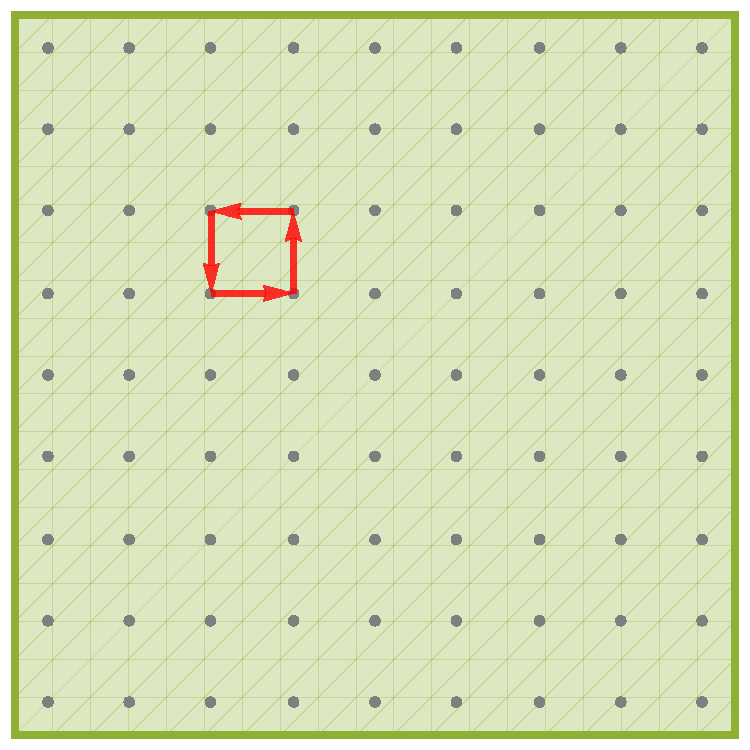
\includegraphics[width=0.5\columnwidth]{appendix/loop}
\caption{二维离散化参数空间中构造 Wilson 环路的示意图。数字标记环路中的顺序。}\label{fig:topoml-appendix}
\end{figure}

\begin{enumerate}

\item 计算每个边上相邻格点上波函数的内积,具体如下,引入
\begin{align}
U_{21} &= V^{\dagger}(\vect{k}_2) V(\vect{k}_1) \\ 
U_{32} &= V^{\dagger}(\vect{k}_3) V(\vect{k}_2) \\ 
U_{43} &= V^{\dagger}(\vect{k}_4) V(\vect{k}_3) \\ 
U_{14} &= V^{\dagger}(\vect{k}_1) V(\vect{k}_4) 
\end{align}

\item 定义 $\mathcal{U}_{ij} = \text{diag}(U_{ij})$,即取出矩阵$U_{ij}$的对角线元素构造对角矩阵,$(\mathcal{U}_{ij})_{mn}:=\delta_{mn}(U_{ij})_{nn}$。

\item 引入 $T_{\text{loop}}(\vect{k}_1) = \mathcal{U}_{14}\mathcal{U}_{43}\mathcal{U}_{32}\mathcal{U}_{21}$,则该由 $\vect{k}_1$ 所标记的方块上第 $n$ 个能带的 Berry 曲率 $\mathcal{F}_{xy}^{(n)}(\vect{k}_1)$ 被定义(计算)为:
\begin{align}
\theta(\vect{k}) = -i \log(T_{\text{loop}}(k_i, k_j))_{nn}\; ,
\qquad    
\mathcal{F}_{xy}^{(n)}(\vect{k}) = \theta(\vect{k}) / s(\vect{k})
\end{align}
$\theta$ 即所谓固体角。

\end{enumerate}

\item Chern 数即为所有方块上固体角之和。即,第 $n$ 个能带的 Chern 数 $c_n$ 由下式得到:

\begin{align}
c_n &= \frac{1}{2\pi} \sum_{i=1}^{L\times L} \theta(\vect{k}_i) \notag \\ 
&= \frac{1}{2\pi}\sum_{i=1}^{L}\sum_{j=1}^{L} -i \log T_{\text{loop}}^{(nn)}(k_i, k_j)
\end{align}

\end{enumerate}

以上即离散化 Chern 数的定义与算法。可以证明,这样定义/计算的 Chern 数具有量子化、规范不变的性质,且当离散化比较大时即能重现连续版本的 Chern 数值。




\begin{theorem}
上述算法计算的 Chern 数一定为整数。
\end{theorem}

\begin{proof}
考虑某一具体的能带,某一方块上 Wilson 环路四条边上两端的本征态的内积简记作 $\langle1|4\rangle$, $\langle4|3\rangle$, $\langle3|2\rangle$, $\langle2|1\rangle$,则
\begin{align}
\theta &= -i\log (\langle1|4\rangle\langle4|3\rangle\langle3|2\rangle\langle2|1\rangle) \\ 
&= (-i\log \langle1|4\rangle + -i\log \langle4|3\rangle + -i\log \langle3|2\rangle + -i\log \langle2|1\rangle) + 2m\pi
\end{align}
其中 $m$ 为某一整数。
而 Chern 数等于所有 plaquette 上这样的 $\theta$ 之和。注意到,每个 link 上会做两次内积且方向相反,也就是说,例如 $\langle3|2\rangle$ 和 $\langle2|3\rangle$ 各有一次。而这两者是互为共轭的,对于确定好的割线,这两个复数的相角是互为相反数的,也即,
\begin{align}
-i\log \langle3|2\rangle + -i\log\langle2|3\rangle = 0
\end{align}
其他 link 类似。因此,对最后计算出来的 Chern 数有
\begin{align}
c_n = \frac{1}{2\pi}\sum \theta = 0 + \frac{1}{2\pi}(2n\pi) = n
\end{align}
$n$ 为某一整数。证毕。
\end{proof}


\begin{theorem}
上述算法计算的 Chern 数与波函数所选取的规范无关。
\end{theorem}

\begin{proof}
对波函数做一个任意的规范变换,
\begin{align}
|u(\vect{k})\rangle \rightarrow |\tilde{u}(\vect{k})\rangle = e^{\ii\chi(\vect{k})}|u(\vect{k})\rangle
\end{align}
$\chi(\vect{k})$ 为一任意相位,则
\begin{align}
\tilde{T} 
&= \langle\tilde{u}(\vect{k}_1)|\tilde{u}(\vect{k}_4)\rangle\langle\tilde{u}(\vect{k}_4)|\tilde{u}(\vect{k}_3)\rangle\langle\tilde{u}(\vect{k}_3)|\tilde{u}(\vect{k}_2)\rangle\langle\tilde{u}(\vect{k}_2)|\tilde{u}(\vect{k}_1)\rangle \\
&= \langle u(\vect{k}_1)|u(\vect{k}_4)\rangle\langle u(\vect{k}_4)|u(\vect{k}_3)\rangle\langle u(\vect{k}_3)|u(\vect{k}_2)\rangle\langle u(\vect{k}_2)|u(\vect{k}_1)\rangle \nonumber\\
& \quad \times e^{\ii[\chi(\vect{k}_1)-\chi(\vect{k}_2)+\chi(\vect{k}_2)-\chi(\vect{k}_3)+\chi(\vect{k}_3)-\chi(\vect{k}_4)+\chi(\vect{k}_4)-\chi(\vect{k}_1)]} \\ 
&= \langle u(\vect{k}_1)|u(\vect{k}_4)\rangle\langle u(\vect{k}_4)|u(\vect{k}_3)\rangle\langle u(\vect{k}_3)|u(\vect{k}_2)\rangle\langle u(\vect{k}_2)|u(\vect{k}_1)\rangle \\
&= T
\end{align}
因此 $\tilde{\theta} = \theta$ 不变。Chern 数计算结果不变。
即该算法具有规范不变性。证毕。
\end{proof}

% \begin{proof}
% 容易验证,对任意 $\vect{k}$ 点处的波函数乘任意相角,牵涉到该点的 plaquette 上的 Berry 曲率不变。例如,
% \begin{align}
% |\tilde{3}\rangle = e^{i\chi} |3\rangle
% \end{align}
% 则
% \begin{align}
% \langle1|4\rangle\langle4|\tilde{3}\rangle\langle\tilde{3}|2\rangle\langle2|1\rangle 
% &= \langle1|4\rangle\langle4|e^{i\chi}|3\rangle\langle3|e^{-i\chi}|2\rangle\langle2|1\rangle \\
% &= \langle1|4\rangle\langle4|3\rangle\langle3|2\rangle\langle2|1\rangle
% \end{align}
% 即 $\tilde{\theta} = \theta$ 不变。因此,对任意 $\vect{k}$ 取任意规范 Chern 数计算结果不变。即该算法具有规范不变性。证毕。
% \end{proof}

\begin{theorem}
上述算法得到的 Berry 曲率,其离散化很大的极限($L\rightarrow\infty$,$\Delta k\rightarrow0$)等于连续版本的 Berry 曲率;对于没有很奇异的情况的模型,有限离散化的 Chern 数计算结果就可以完全准确地得到 连续的 Chern 数结果。
\end{theorem}

\begin{proof}
易验证\footnote{这里为简化记号,不致混淆的情况下以 $(x,y)$ 代记 $(k_x,k_y)$。}:
\begin{align}
\langle u(\vect{k}_2)|u(\vect{k}_1)\rangle 
&= \langle u(x_{i+1},y_j)|u(x_i,y_j)\rangle \\ 
&= (\langle u(x_i,y_j)| + \Delta k_x\langle\partial_xu(x_i,y_j)|)|u(x_i,y_j)\rangle \\ 
&= 1 + \Delta k_x \langle\partial_xu(x_i,y_j)|u(x_i,y_j)\rangle \\ 
&= 1 - \Delta k_x \langle u(x_i,y_j)|\partial_xu(x_i,y_j)\rangle \\
&\rightarrow 1 + \ii \int_1^2A(x_i,y_j)d\vect{k}_x
\end{align}
因此有
\begin{align}
\lim_{\Delta k\rightarrow0} T_{\text{loop}}^{(nn)}(x_i,y_i) = 
1 + \ii \oint_{\square} \vect{A}(\vect{k})\cdot d\vect{k} = e^{\ii\theta(\vect{k}) S_{\square}} 
\end{align}
其中,$S_{\square}$ 为方块面积。$\theta(\vect{k})$ 即连续版本的 Berry 曲率。定理前半部分证毕。

定理后半部分:当没有“很”奇异的情况时\footnote{很奇异的情况,如 Berry curvature 发散},有限离散化即可完全准确重现(算出)连续版本的 Chern 数,这个有限离散化的下界 $L_0$ 由 Berry 场中最奇异(绝对值最大)的一点 $\theta_m$ 决定:
\begin{align}
\left(\dfrac{2\pi}{L_0}\right)^2 \sim \dfrac{\pi}{\theta_{m}}
\end{align}
$L$ 比 $L_0$ 大很多时即可认为算法完全有效(完全准确)。
\footnote{读者可以想一想为什么。}
\end{proof}







注意,以上三个定理体现出该算法的强大性。比起连续版本下通过解析计算的复杂与极端情况下(如某处具有很奇异的 Berry 曲率时)的不准确,该算法不但简单,易算,速度快\footnote{经测试离散化到 $100\times100$ 时计算 Haldane 模型的 Chern 数只需 秒的量级(python3, Mathematica)},而且准确,鲁棒。实际运行代码时,只有当遇到能隙关闭(gapless)的情况时可能会给出非整数的结果\footnote{对于这种情况,需要说明的是,上述定理1并未被违反,出现非整数的情况是由于实际计算中机器精度的问题。具体来说,当遇到能带简并的情况时,程序有可能在临近的某两个点对角化得到的波函数内积为0,或无限趋近于0,内积为0本身是没有问题的,但由于计算机机器精度的存在,可能会给存储的数本身附加上一个很小的实部和虚部,而这会引入任意的相角。理论上讲,一个有序的link上的内积和它的反向内积得到的数应互为共轭,但此时由于两者都被引入了任意相角,可能不再共轭,这就是会使最后算得的Chern数不为整数的来源。这个问题本身可以通过对程序做一些优化来避免。但仍需注意,gapless 情况本身就不应该计算 Chern 数。}——而这种情况本是不被允许计算 Chern 数的\footnote{能隙关闭的情况下,能隙关闭的点上能级是简并的,无法定义哪个态属于那个能带\cite{topobook}。这样的情况也恰好是不同拓扑相相变的边界。}。


对于该 Chern 数算法,我们开发了专门的程序包,分别基于 python3 语言和基于 Wolfram Mathematica 语言(v11.3)。开源地址\cite{repo-chern} https://github.com/atom-sun/chern。
